\section{Konzept}\label{sec:konzept}
Dieses Kapitel stellt das Konzept zur Realisierung des Projekts vor. 
Dies umfasst den allgemeinen Systemaufbau, sowie Architekturentwürfe hinsichtlich der Server- und Clientseite inklusive den im Verbund eingesetzten Softwaremodulen.
\subsection{Systemaufbau}\label{sec:sysaufbau}
Das System soll in eine Server- und Clientseite aufgeteilt sein. 
Da es sich um eine Webapplikation handeln soll, wird die Interaktion mit dem Server über einen Webbrowser stattfinden und dieser soll auch gleichzeitig der Client sein. Für Aufgaben wie das Starten des Servers, soll die Steuerung über die Kommandozeile des Host-Computers möglich sein. Alle anderen Interaktionen werden über den Web-Clients ausgeführt.
\subsection{Netzwerkaufbau}\label{sec:netzwerkaufbau}
Als Kommunikationsprotokoll soll das aus dem Webbereich bekannte HTTP resp. HTTPS Protokoll zum Einsatz kommen. Der Server wird als Webserver fungieren, Anfragen müssen vom Client aus initiiert werden (vgl. Abschnitt \ref{sec:www}). Bei Parts, welche Echtzeitinteraktion benötigen, soll das Websocket (ws) Protokoll zum Einsatz kommen, welches eine bidirektionale Kommunikation zwischen Server und Client ermöglicht. Der Server soll sowohl in einem Intranet wie auch im Internet lauffähig sein. Dabei kann er, je nach infrastruktureller Realisierung über ein IPv4 oder IPv6 Adresse erreicht werden, bei Nutzung eines DNS-Servers auch über eine Domain.\\ \\

Der Kommunikationsaufbau ist schematisch in Abbildung \ref{fig:server_kommdiagram} dargestellt. 

\begin{figure}[H]
	\centering
	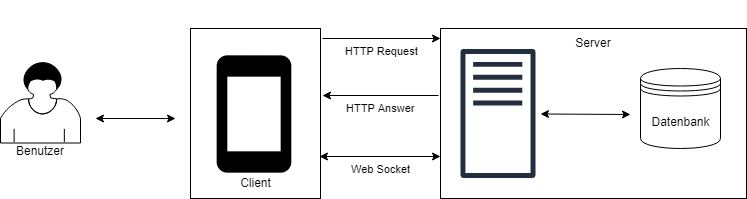
\includegraphics[width=0.8\linewidth]{bilder/server_diagram}
	\caption[Kommunikationsaufbau des zu entwickelnden Systems]{Kommunikationsaufbau des zu entwickelnden Systems}
	\label{fig:server_kommdiagram}
\end{figure}


\subsection{Entwurf des Servers}\label{sec:serverkonzept}
Aufbauend auf das Grundlagen- und Analysekapitel sollen in diesem Abschnitt die Lösungen hinsichtlich der Serverkomponente des Projekts aufgezeigt werden. 
\subsubsection{Laufzeitumgebung: Node.js}\label{sec:nodejs}
Als Laufzeitumgebung und Grundbaustein des Servers wird die JavaScript-""Laufzeitumgebung \emph{Node.js} \cite{Node.js} genutzt werden, da dies zwei wesentliche Vorteile mit sich bringt:
\begin{enumerate}
	\item \emph{Node.js} nutzt als Paketmanager und Projektverwaltungstool \emph{Node Paket Manager} (NPM). Mit dieser Software ist der Zugang zu über 350.000~Paketmodulen (Stand 13. Januar 2017) \cite{npm2017} gegeben und diese können das Projekt Modular erweitern. Diese können in \emph{Node.js} gemäß dem IoC Prinzips genutzt werden (siehe auch Abschnitt \ref{sec:wafs}). 
	Ebenso können mit NPM grundlegende Start- und Installationsskripte leicht ausgeführt werden. 
	\item Da \emph{Node.js} eine JavaScript-Laufzeitumgebung ist, wird zur Programmierung die Skriptsprache \emph{JavaScript} genutzt, welche auch auf der Clientseite im Webbrowser zum Einsatz kommt. Dies erleichtert den Implementierungsprozess, da einheitlich in einer Sprache geschrieben wird.
\end{enumerate}
Darüber hinaus können NPM-Pakete auch auf der Clientseite genutzt werden (siehe dazu auch Abschnitt \ref{sec:browserify}). Eine gute Skalierbarkeit ist ebenfalls gegeben. Dies wird in folgenden Abschnitten genauer erläutert. Ist ein besonders hoher Ressourcenbedarf von Nöten (z.B. eine Bildungseinrichtung möchte einen zentralen Server installieren, welche viele Klassen/Kurse bedienen soll) können mehrere Serverinstanzen auf einem Computer parallel laufen und vorab mit einem Lastenverteiler (Load Balancer) Server, wie z.B. \emph{NGINX} verwaltet werden. Um dies zu erreichen wird das Projekt mit \emph{Node.js} realisiert werden und nicht mit einem \emph{php}-Framework. \\ Da \emph{Node.js} grundlegend sehr offen ist was seinen Einsatzzweck betrifft, soll als Webserver Modul das NPM-Modul \emph{Express} genutzt werden, welches im nächsten Abschnitt genauer erläutert wird.
\subsubsection{Webserver: Express}\label{sec:expressjs}
Um mit Node.js komfortabel eine Webapplikation zu implementieren, soll das bekannte Webserver-Framework \emph{Express} eingesetzt werden, welches viele HTTP-""Dienstprogrammmethoden und den Einsatz von Middlerwarefunktionen gestattet. Hierbei wird jeder eingehende HTTP Anfrage von Funktion zu Funktion weitergeleitet (Aufruf der Methode \texttt{next()}) oder explizit beantwortet (die Funktion besitzt ein Rückgabewert). Ebenso ist mit \emph{Express} das Abbilden von Routen möglich. \emph{Express} wird für den gesamten administrativen Teil des Lehrer-Login zum Einsatz kommen. Ebenso soll durch \emph{Express} das Anlegen und Editieren von Lehreinheiten möglich sein (vgl. Sektion \ref{sec:sysbeschreib}). 
Da für den gesamten Lehrer-Backendbereich \emph{Express} zum Einsatz kommen soll und hier mit einfachen HTTP-Requests gearbeitet wird, kann der Einsatz von JavaScript auf der Client-Seite auf ein Minimum reduziert werden, was dem Einsatz auf Servereinheiten mit nicht modernen Webbrowsern entgegenkommt (sollte Client und Server auf der gleichen Maschine ausgeführt werden).\\ \\ 
Für den interaktiven Part des Projekts werden zur Kommunikation \emph{WebSockets} genutzt, welche mithilfe der JavaScript-Bibliothek \emph{Socket.IO} realisiert werden sollen. Dies wird in der nächsten Sektion beschrieben.   

\subsubsection{Socket.IO}\label{sec:socketio}
Die JavaScript-Bibliothek \emph{Socket.IO} \cite{Socket.IO2019} ermöglicht bidirektionale Echtzeit-\\Kommunikation zwischen Webclient und Server, wobei jeweils ein Bibliotheksteil auf Server- und Clientseite zum Einsatz kommt. Ein großer Vorteil ist, dass beide Komponenten eine nahezu identische API aufweisen. Daten können sehr einfach von Client ereignisgetrieben (event-driven) zwischen Server und Client sowie vice versa ausgetauscht werden. Client und Server lauschen dabei gegenseitig auf Ereignisse, wie das Verbinden eines neuen Clients oder auch selbst implementierte Ereignisse. Dabei können jegliche \emph{JavaScript} Daten hin-und hergeschickt werden. Eine händische Konvertierung in das JSON-Format ist nicht notwendig. \emph{Express} wird zunächst Client Daten (HTML-, CSS- und JS- Daten) auf einer festgelegten Route senden. Anschließend wird die Kommunikation von \emph{Socket.IO} gesteuert. 
\subsubsection{Sonstige Module}
Neben \emph{Express} ist der Einsatz von weiteren Modulen (\emph{Node Packages}) vorgesehen, welche unterschiedliche Funktionen realisieren sollen. Diese sind:
\begin{itemize}
	\item \textbf{Body-Parser}: Diese Modul ermöglicht das einfach Auslesen von HTTP-Requests. Schickt ein Client bspw. Formulardaten, können diese einfach gelesen und ausgewertet werden. 
	\item \textbf{express-session}: Da Lehrende und Administratoren zur Nutzung der Software einen gültigen Zugang besitzen müssen, sind zur Authentifizierung der Nutzenden HTTP-Sessions vorgesehen (vgl.  Abschnitt\ref{sec:www}). Das Modul \emph{Express-Session} macht das Arbeiten mit diesen sehr komfortabel. Über das Zusatzmodul \emph{connect-session-sequelize} ist die Zusammenarbeit mit der gewählten Datenbank einfach. (Weiterführende Informationen diesbezüglich im Abschnitt \ref{sec:datenbank} \hyperref[sec:datenbank]{Wahl der Datenbank}). 
	\item \textbf{Pug}: Die Template Engine \emph{Pug} besitzt seine eigene Syntax und macht das Entwerfen und Schreiben von HTML Templates sehr komfortabel. Zusätzlich werden Funktionalitäten wie Vererbung und Mixins unterstützt. Eine Einsatzbeschreibung erfolgt in Kapitel \ref{sec:implementierung} \hyperref[sec:implementierung]{Implementierung}. Pug soll für sämtliche zu übertragende HTML Dokumente genutzt werden.   
\end{itemize}

Neben den o.g. Modulen kommen noch weitere zum Einsatz, welche kleinere Funktionen realisieren. Diese wurden aus Gründen der Übersicht hier nicht gelistet, werden aber in der Datei \texttt{package.json} des Projekt-Quellcodes gelistet sein.
\subsubsection{Wahl der Datenbank}\label{sec:datenbank}
Da bei dem zu entwickelnden System vielerlei Daten anfallen, wie registrierte Nutzer, angelegte Kurse, interaktive Unterrichtseinheiten und mehr, ist der Einsatz eines Datenbanksystems unerlässlich. Grundlegend können Datenbanksysteme in zwei Kategorien unterteilt werden: 
\textbf{SQL} und \textbf{noSQL} Systeme. \\ \\ SQL Systeme speichern ihre Daten in sogenannten Relationsmodellen, welche als Tabelle visualisiert werden können. Hierbei beschreibt der Tabellenkopf den Datensatz und den Datentypus (jede Spalte für sich), während Zeilen eine Entität (Eintrag) in der Datenbank beschreiben. Vorteil hierbei ist, dass die Daten konform sind, d.h. jeder Zugriff liefert immer einen Rückgabewert \cite{neumann2015entwicklung}. Nachteil ist der erhöhte Aufwand, sollte die Definition des Relationsmodells im Nachhinein geändert werden, was das Aktualisieren sämtlicher Daten erfordern würde. Desweiteren sind SQL System schwer skalierbar, da für größere Datenbanksysteme leistungsstärkere Server gekauft werden müssen. Mehrere Relationsmodelle können über Fremd-Schlüssel (Querverweise) miteinander verbunden werden, um auch komplexere Sachverhalte abbilden zu können. \\ \\ NoSQL Systeme lassen sich nach Speicher-Arbeitsweise in verschiedene Subkategorien einteilen \cite{neumann2015entwicklung}. Oft genutzt sind die Typen Dokumentenorientiert, Key-Value Pairs (Schlüssel-Wert Paare) und Graphen-basierte Systeme. Dokumentenorientierte NoSQL Datenbanken legen pro Entität ein Dokument an, in welchem die Informationen meist im JSON Format abgespeichert werden. Key-Value Systeme verfolgen ein einfaches Zuordnungsprinzip und bilden Schlüssel-Wert Paare, ähnlich einer Dictionary Datenstruktur. Bei Graphen-basierten Systemen werden Entitäten und ihre Beziehungen untereinander an sich gespeichert. Generell sind NoSQL Systeme weniger statisch im Vergleich zu SQL Systemen. Dies räumt eine große Flexibilität beim Speichern von Daten ein, da Datensätze auch unvollständig gespeichert werden können. Dies kann auch als Nachteil interpretiert werden, ist aber generell immer vom Kontext des Projekts abhängig. \\ \\    
Für das zu entwickelnde System soll ein möglichst flexibler Weg gewählt werden was die Wahl der Datenbank betrifft. Da das MVC-Prinzip zum Einsatz kommen soll, beschreibt der Model-Teil von zu bereitstellenden Daten auch wie diese über welche Funktionalität aus der Datenbank geladen werden sollen. Der Controller soll nur die vom Model bereitgestellten Funktionen nutzen und keine direkten Datenbankzugriffe selbst tätigen. Damit die Software im hohem Maße skalierbar bleibt, ist der Einsatz eines sogenannter Object-Relationship-Mapper, kurz ORM, vorgesehen, welcher an verschiedenste Datenbanksysteme angebunden werden kann. Da das Projekt in seiner kleinsten Skalierung lokal auf einem Einplantinencomputer wie dem \emph{Raspberry Pi 3} und lokal im Intranet laufen können soll, ist für den Anfang die Verwendung eines Datenbanksystems vorgesehen, welches vollständig durch eine Programmbibliothek abgebildet ist. Dies hat den Vorteil, dass kein extern laufendes Datenbanksystem installiert, gewartet und gestartet werden muss, da die komplette Datenbank in einer einzigen Datei auf dem Server gespeichert wird. Diese Anforderungen erfüllt die Programmbibliothek \emph{SQLite}~\ref{SQLiteConsortium2019}. Die gesamte Datenbank kann hier sogar rein im Arbeitsspeicher gehalten werden, was jedoch den Nachteil mit sich bringt, dass bei einem Ausfall oder Abschalten des Server der kompletten Verlust sämtlicher Daten folgt. 
\\ Als ORM wird auf das NPM Modul \emph{Sequelize}, welches neben \emph{SQLite} mit viele andere bekannte SQL Datenbanksystemen zusammenarbeiten kann, u.A. \emph{Postgres}, \emph{MariaDB} und \emph{Microsoft SQL Server}~\cite{Depold2019}. Der Wechsel auf ein anderes SQL Datenbanksystem ist somit jederzeit problemlos möglich, falls gewünscht. \\ \\  
Das Zusatzmodule \texttt{connect-session-sequelize} ermöglicht eine einfache Handhabung der Session-Verwaltung von Lehrenden, die in das System eingeloggten sind. Dazu werden entsprechende Tabellen zur Verwaltung der Sessions und deren Lebenszeit automatisch via \emph{Sequelize} in der Datenbank angelegt. Zuvor sollen die Passwörter sicher gespeichert werden, d.h. nicht im Klar-Text, sondern nur als Hashwerte, welche zusätzlich mit einem Salt verstärkt werden\footnote{Weiterführende Informationen unter:  \texttt{https://de.wikipedia.org/wiki/Salt\_(Kryptologie)}}.

Da zum Zeitpunkt der Recherche kein zu \emph{SQLite} ähnliches und für den produktiven Einsatz lauffähiges NoSQL Äquivalent gefunden werden konnte, fiel die Entscheidung auf SQLite. Die genannten Vorteile eines NoSQL Systems scheinen für die Anforderungen des zu entwickelenden Systems ohnehin nicht relevant, obgleich sogar ein Umstieg auf NoSQL Datenbkansystem möglich wäre, auch wenn dies mit einem etwas erhöhten Aufwand verbunden wäre, da dann auch der ORM gewechselt und die Models entsprechend angepasst werden müssten.  

\subsubsection{Server Architekturdiagramm}\label{sec:serverarchitekt}
Zusammenfassend lässt sich der finale Entwurf der Serverarchitektur in folgender Abbildung \ref{fig:server_diagram} visualisieren. Er wird in Kapitel {\ref{sec:implementierung} Implementierung} umgesetzt.

\begin{figure}[H]
	\centering
	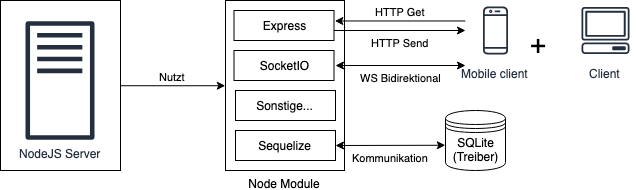
\includegraphics[width=0.8\linewidth]{bilder/server_architektur}
	\caption[Aufbau der geplanten Serverarchitektur]{Aufbau der geplanten Serverarchitektur}
	\label{fig:server_diagram}
\end{figure}
\footnotesize \underline{Hinweis:} NodeJS Module aus der Sektion \textbf{Sonstige Module} wurden aus Gründen der Übersicht in dieser Grafik nicht abgebildet.

\normalsize 
\newpage
\subsection{Entwurf des Clients}\label{sec:clientkonzept}
Wie zuvor in Abschnitt \ref{sec:sysbeschreib} erörtert, ist es vorgesehen drei verschiedene Clients zu implementieren, welche alle auf dem gleichen Prototyp basieren sollen, allerdings verschiedene Zwecke verfolgen. Ein Webclient jeweils für \textbf{Lehrende/Dozierende}, \textbf{Schülerinnen und Schüler} und einen für \textbf{Großbildanzeigen} optimierten wie Projektoren o. Ä. vor. Zur Vereinfachung werden diese gemäß der vorherigen Reihenfolge \textbf{Teacher Client}, \textbf{Student Client} und \textbf{Presenter Client} in diesem und darauffolgendem Kapitel genannt.

\subsubsection{User Interface}\label{sec:uientwurf}
Da das Projekt als Web-Applikation implementiert werden soll, wird das UI gänzlich durch die Stylesheet-Sprache \emph{CSS} beschrieben. Im Jahr 2018 wurden erstmals häufiger mobile Endgeräte wie Smartphones zur Internetnutzung herangezogen als klassische Computer oder Laptops \cite{Rabe2019}. Viele Design-Frameworks setzen daher schon länger auf das Prinzip "`Mobile First"'. Die Applikation soll letztlich sowohl auf Computern und Smartphones aber auch Großbildgeräten angezeigt werden. Ein Web-Design-Framework als Basis, welches bereits viele relevante Web-Design Standards wie das o.g. "`Mobile First"' berücksichtigt, bildet ein solides Fundament in Sachen Usability (Software-Ergonomie) und UI-Design. Eines der populärsten dieser Art ist \emph{Bootstrap}, welches zusammen mit einem frei erhältlichen Design-Theme von \emph{FreeHTML5.co} \cite{FreeHTML5.co2019} genutzt werden soll. Das gewählte Theme soll an die Applikation angepasst und teils für die Großbild Anzeige des Presenter Clients optimiert werden.  
\subsubsection{Browserify}\label{sec:browserify}
Um das Nutzen von NPM Modulen und die damit verbundene \texttt{require()} Funktionalität auch auf der Clientseite zu ermöglichen, soll die Bundle-Soft\-ware~\emph{Brow\-serify}~\cite{Browserify2019} zum Einsatz kommen. Mit ihr können alle Module, welche über den \emph{Node Package Manager} in das Projekt hinzugefügt wurde im Webbrowser des Clients genutzt werden. Dazu bündelt die Bibliothek alle Module und stellt anschließend eine einzige JS-Datei zur Verfügung, die nur noch im HTML-Dokument eingebunden werden muss. Mithilfe der \texttt{require()} Funktionalität, welche eigentlich nur in der \emph{Node.js} Umgebung genutzt werden kann, ist es möglich den Code übersichtlicher in mehrere Dateien/Module aufzuteilen. Dies war früher ohne Aufwand auf der Browser-Seite nicht möglich, ist aber durch die Einführung von Modulen seit ECMAScript\footnote{Der als ECMAScript (ECMA 262) standardisierte Sprachkern von JavaScript beschreibt eine dynamisch typisierte, objektorientierte, aber klassenlose Skriptsprache. (Wikipedia.org)} in Version 6 nun möglich. Oftmals wird aber aus Kompatibilitätsgründen zu älteren Webbrowsern auf Lösungen wie \emph{Browserify} gesetzt. Zusätzlich kann Software wie \emph{Babel} den geschriebenen \emph{JavaScript} Code so übersetzen, dass er auch von älteren Webbrowsern interpretiert wird (auch Transpiler genannt). Sämtliche folglich genannten NPM Module resp. Bibliotheken sollen via \emph{Browserify} in eine \emph{JavaScript} Datei zusammengefasst werden und anschließend pro Client eingebunden werden. Das bringt den zusätzlichen Vorteil, dass für jegliches, auf Browser-Seite eingesetztes JavaScript nur ein einziger HTTP-Get Request für den Code benötigt wird, da wie erwähnt nur eine \emph{JavaScript} Datei pro Client angefordert werden muss. 
\subsubsection{JavaScript Lösungen}\label{sec:clientjs}
Von folgenden JavaScript Lösungen soll auf der Clientseite Gebrauch gemacht werden, um den Implementierungsprozess zu optimieren:
\begin{itemize}
	\item \textbf{VueJS}: Um das Anzeigen, Editieren und Anpassen dynamischer Inhalte zu erleichtern, soll das JS-Webframework \emph{VueJS} \cite{You2019} zum Einsatz kommen, da dieses gut skalierbar ist und alle benötigten Funktionalitäten mit sich bringt. Im Vergleich zu \emph{AngularJS} und \emph{React} (siehe auch Abschnitt \ref{sec:clientseitigeransatz}), biete \emph{VueJS} eine flachere Lernkurve und kann als ein guter Kompromiss aus seinen zwei Konkurrenten betrachtet werden. Mittlerweile hat \emph{VueJS} seinen Konkurrent \emph{React} in Sachen Popularität auf \emph{GitHub} überholt \cite{Daityari2019}. \emph{VueJS} ist auch gemessen an der Dateigröße von nur 80~KB im Vergleich deutlich kleiner als Angular mit 500 KB.
	\item \textbf{Socket.IO}: Das bereits in Abschnitt \ref{sec:socketio} erwähnte \emph{Socket.IO} besitzt ein Bibliotheksteil, welcher auf der Client-Seite im Webbrowser zum Einsatz kommt. Dadurch wird die bidirektionale Kommunikation mit der Server ermöglicht und es soll in beide Richtungen Daten in Echtzeit ausgetauscht werden. 
	\item \textbf{Zingchart}: Zur Visualisierung der Wörterwolke (Word Cloud), welche bei der interaktiven Unterrichtsmethode Brainstorming zum Einsatz kommt, soll die auf diese Szenarien spezialisierte JavaScript Bibliothek \emph{ZingChart} genutzt werden (vgl. Abbildung \ref{fig:wordcloud}). Die Software ist in einer freien Version erhältlich, wobei lediglich stets ein kleines \emph{ZingChart} Logo stets angezeigt wird \cite{zingchartpricing}.
\end{itemize}

\begin{figure}[H]
	\centering
	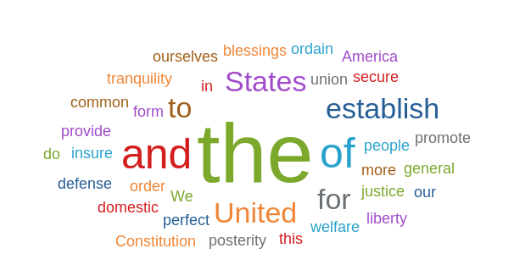
\includegraphics[width=0.8\linewidth]{bilder/wordcloud}
	\caption[ZingChart Word-Cloud]{Eine Word-Cloud/Wörterwolke generiert durch ZingChart \cite{ZingSoft2019}}
	\label{fig:wordcloud}
\end{figure}

\subsubsection{Client Architekturdiagramm}\label{sec:clientarchitekt}
Nachfolgend die umzusetzende Architektur der Client-Anwendung. 

\begin{figure}[H]
	\centering
	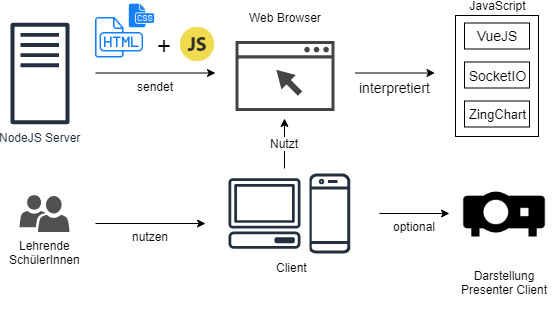
\includegraphics[width=0.8\linewidth]{bilder/client_architektur}
	\caption[Aufbau der geplanten Client Architektur]{Aufbau der geplanten Client Architektur}
	\label{fig:client_diagram}
\end{figure}
\footnotesize \underline{Hinweis:} Zum besseren Verständnis wurden die Rollen des Servers und der Nutzer ebenso dargestellt. Der Presenter Client nutzt in der Grafik ein Projektor. Dies ist eine Option und nicht zwingend von Nöten. Alle Clients können auf dem gleichem Server-Host Computer ausgeführt werden (z.B. in unterschiedlichen Tabs eines Webbrowsers) als auch auf separaten Endgeräten. 



\normalsize
